\bta{超重和失重现象}

\begin{enumerate}[leftmargin=0em]
\renewcommand{\labelenumi}{\arabic{enumi}.}
% A(\Alph) a(\alph) I(\Roman) i(\roman) 1(\arabic)
%设定全局标号series=example	%引用全局变量resume=example
%[topsep=-0.3em,parsep=-0.3em,itemsep=-0.3em,partopsep=-0.3em]
%可使用leftmargin调整列表环境左边的空白长度 [leftmargin=0em]
\item
\exwhere{$ 2011 $年理综天津卷}
某同学利用测力计研究在竖直方向运行的电梯运动状态,他在地面上用测力计测量砝码的重力,示数是$ G $,他在电梯中用测力计仍测量同一砝码的重力,发现测力计的示数小于$ G $,由此判断此时电梯的运动状态可能是 \tk{减速上升或加速下降} 。



\item 
\exwhere{$ 2015 $年江苏卷}
一人乘电梯上楼,在竖直上升过程中加速度 $ a $ 随时间 $ t $ 变化的图线如图所示,以竖直向上为 $ a $ 的正方向,则人对地板的压力 \xzanswer{AD}
\begin{figure}[h!]
\centering
\includesvg[width=0.23\linewidth]{picture/svg/481}
\end{figure}


\fourchoices
{$ t= $ $ 2 $ $ s $ 时最大}
{$ t= $ $ 2 $ $ s $ 时最小}
{$ t= $ $ 8.5 $ $ s $ 时最大}
{$ t= $ $ 8.5 $ $ s $ 时最小}



\item 
\exwhere{$ 2018 $年浙江卷($ 4 $月选考)}
如图所示,小芳在体重计上完成下蹲动作。下列$ F-t $图像能反映体重计示数随时间变化的是 \xzanswer{C}


\begin{figure}[h!]
\centering
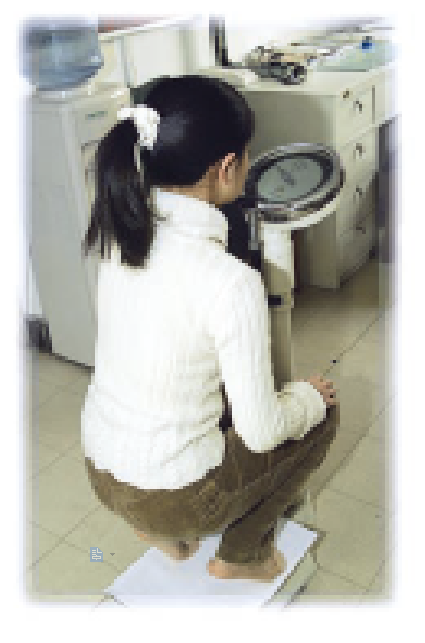
\includegraphics[width=0.15\linewidth]{picture/screenshot001} \quad 
\includesvg[width=0.83\linewidth]{picture/svg/482}
\end{figure}



\item 
\exwhere{$ 2012 $年理综山东卷}
将地面上静止的货物竖直向上吊起,货物由地面运动至最高点的过程中,$ v-t $ 图像如图所示。以下判断正确的是 \xzanswer{AC}
\begin{figure}[h!]
\centering
\includesvg[width=0.23\linewidth]{picture/svg/483}
\end{figure}

\fourchoices
{前$ 3\ s $内货物处于超重状态}
{最后$ 2\ s $内货物只受重力作用}
{前$ 3\ s $内与最后$ 2\ s $内货物的平均速度相同}
{第$ 3\ s $末至第$ 5\ s $末的过程中,货物的机械能守恒}

\item 
\exwhere{$ 2016 $年上海卷}
在今年上海的某活动中引入了全国首个户外风洞飞行体验装置,体验者在风力作用下漂浮在半空。若减小风力,体验者在加速下落过程中 \xzanswer{B}


\fourchoices
{失重且机械能增加}
{失重且机械能减少}
{超重且机械能增加}
{超重且机械能减少}





\item 
\exwhere{$ 2014 $年理综北京卷}
应用物理知识分析生活中的常见现象,可以使物理学习更加有趣和深入。例如平伸手掌托起物体,由静止开始竖直向上运动,直至将物体抛出。对此现象分析正确的是 \xzanswer{D}

\fourchoices
{手托物体向上运动的过程中,物体始终处于超重状态}
{手托物体向上运动的过程中,物体始终处于失重状态}
{在物体离开手的瞬间,物体的加速度大于重力加速度}
{在物体离开手的瞬间,手的加速度大于重力加速度}


\item 
\exwhere{$ 2015 $年理综重庆卷}
若货物随升降机运动的$ v-t $图像如图所示(竖直向上为正),则货物受到升降机的支持力$ F $与时间$ t $关系的图像可能是 \xzanswer{B}
\begin{figure}[h!]
\centering
\includesvg[width=0.9\linewidth]{picture/svg/484}
\end{figure}

\item 
\exwhere{$ 2015 $年海南卷}
如图,升降机内有一固定斜面,斜面上放一物体,开始时升降机做匀速运动,物块相对斜面匀速下滑,当升降机加速上升时 \xzanswer{BD}
\begin{figure}[h!]
\centering
\includesvg[width=0.15\linewidth]{picture/svg/485}
\end{figure}

\fourchoices
{物块与斜面间的摩擦力减小}
{物块与斜面间的正压力增大}
{物块相对于斜面减速下滑}
{物块相对于斜面匀速下滑}








\end{enumerate}



